\documentclass[11pt,spanish,b5paper]{book}
\usepackage[T1]{fontenc}
\usepackage{selinput}
\SelectInputMappings{%
  aacute={á},
  ntilde={ñ}
}
\usepackage{babel}
\usepackage{tipa}
\usepackage{titlesec}
\usepackage{footnote}
\usepackage{amsmath}
\usepackage{enumerate}
\usepackage{chngcntr}
\usepackage{emptypage}
\usepackage{graphicx}
\usepackage{extarrows}
\counterwithout{footnote}{chapter}
\counterwithout{subsection}{section}

\usepackage{fancyhdr}
\setlength{\headheight}{15pt}

\pagestyle{fancy}

\fancyhf{}
\fancyhead[LE,RO]{\thepage}
\fancyhead[RE,LO]{\thesubsection}
\fancyhead[CO]{EL HABLA PASIEGA}
\fancyhead[CE]{R. J. PENNY}

\fancypagestyle{plain}{ %
  \fancyhf{} % remove everything
  \renewcommand{\headrulewidth}{0pt} % remove lines as well
  \renewcommand{\footrulewidth}{0pt}
}

\renewcommand{\headrulewidth}{0pt}

\usepackage{titlesec} % or RequirePackage[loadonly]{titlesec} in a cls file
\titleformat{\subsection}[runin]{\normalfont\bfseries}{\thesubsection}{3pt}{}
\titleformat{\chapter}[hang]{\Large\bfseries\centering}{{\thechapter}{. }}{0pt}{\large\bfseries}



\newcommand{\uc}{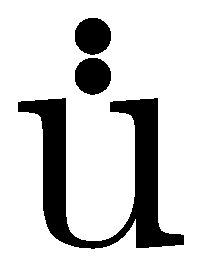
\includegraphics[trim=0.0em 0.15ex 0.0em 0.0em, clip, width=0.50em]{images/chars/u_central.eps}}

\newcommand{\ucs}{\begingroup\setbox0=\hbox{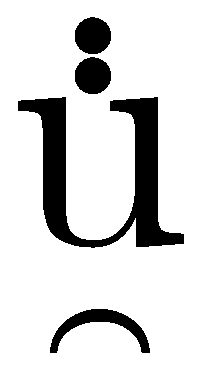
\includegraphics[trim=0em 0.0em 0.0em -1.5em,clip,width=0.50em]{images/chars/u_central_semi.eps}}\parbox{\wd0}{\box0}\endgroup}

\newcommand{\ic}{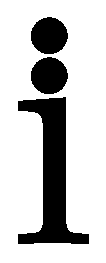
\includegraphics[trim=0.0em 0.15ex 0.0em 0.0em, clip, width=0.215em]{images/chars/i_central.eps}}

\newcommand{\apt}{\begingroup\setbox0=\hbox{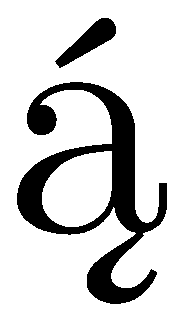
\includegraphics[trim=0em 0.15ex 0.0em 0.0em,clip,width=0.45em]{images/chars/a_palatal_tilde.eps}}\parbox{\wd0}{\box0}\endgroup}

\newcommand{\adp}{\begingroup\setbox0=\hbox{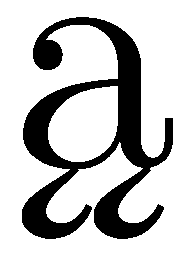
\includegraphics[trim=0em 0.0em 0.0em -4em,clip,width=0.45em]{images/chars/a_doblepalatal.eps}}\parbox{\wd0}{\box0}\endgroup}

\begin{document}
\author{Ralph J. Penny}
\title{EL HABLA PASIEGA: \\ \emph{Ensayo de dialectología montañesa}}
\date{1969}
\maketitle

\titlespacing*{\chapter}{0pt}{0pt}{0pt}

\setcounter{tocdepth}{1}

\renewcommand \thechapter{\roman{chapter}}
\renewcommand \thesection{\Alph{section}}
\renewcommand \thesubsection{§ \arabic{subsection}}

\part*{INTRODUCCIÓN}
\addcontentsline{toc}{part}{INTRODUCCIÓN}

%\begin{figure}[h!]
%  \centering
%    \includegraphics{images/mapa1.png}
%  \caption{Situación geográfica}
%  \label{fig:map1}
%\end{figure}

\chapter{LOS MONTES DE PAS Y SU HABLA}
\section{\emph{Situación geográfica}}
\subsection{} Los montes de Pas se hallan situados en la región sureste de la provincia de Santander (véase mapa 1), en una zona marcadamente montañosa. Se encuentran al este de la carretera nacional Santander-Burgos y comprenden una región compacta de unos 18 kilómetros de este a oeste y  otros tantos de norte a sur. Los ríos que allí bajan de la Cordillera Cantábrica han excavado largos y profundos valles, pero de poca anchura, dejando entre ellos estribaciones altas y abruptas, aunque aprovechables, la mayoría de ellos, para pastos. El clima es generalmente húmedo, y duro en invierno, con bastante nieve, sobre todo en las alturas. 

Las alturas mayores de la zona están representadas, de este a oeste, por Torcaverosa (1561m), Castro Valnera (1707m), Peaña Negra (1498m) y El Colladillo (1416m), que forman la frontera de nuestra comarca con la provincia de Burgos. Dentro del área estudiada, las alturas superan con frecuencia los mil doscientos metros, especialmente en la sierra que separa la cuenca del Miera, al este, de los ríos de Pas y de Pisueña, al oste, siendo corrientes las alturas de novecientos metros en todo el resto de la zona. El lomo de la Braguía, divisoria entre las cuencas del Pas y del Pisueña (véase mapa 1), tiene en su extremo occidental unos setecientos metros de altura, alcanzando unos 1249 al oriente, en su punto de unión con la sierra antes citada. 

Esta configuración del suelo no permite a los ríos la formación anchas cuencas, sino que las constriñe en cauces estrechos, con alguna excepción como en el caso del río Pas. Este río logra formar una llanura de aproximadamente medio kilómetro de ancha en cierta sección de su recorrido, precisamente allí donde hoy se encuentra el pueblo que se llama Vega de Pas. Se cierra inmediatamente después, volviendo a su antigua estrechez. 

Los ríos más considerables son, al este, el Miera, de trazo norte-sur y que no tiene afluentes importantes. Luego el Pas, que en la primera da, parte de su trayecto corre paralelo al Miera, pero que se desvía después a la izquierda para correr de este a oeste, volviendo entonces, ya fuera de nuestra zona, a su curso norte-sur. Sus afluentes, todos a la izquierda son el Yera, el Viaña, el Barcelada, el arroyo de Laral y el río Aldano. Finalmente, al norte del Pas y al oeste del Miera corre el río Pisueña, sin afluente de importancia. Aparte de los ríos mencionados, toda la región abunda en arroyos y fuentes de menor caudal. 

\subsection{} La zona así descrita comprende cuatro municipios: al sur, lindantes con la provincia de Burgos, están San Pedro del Romeral y Vega de Pas; en la parte septentrional están situados Selaya y San Roque de Riomiera (fon.: \textipa{san \=rók\"@ \=rumjér\'5}), también este último, con una pequeña frontera burgalesa. Los límites de esta región son, al sur, la provincia de Burgos (términos de Valdeporres, Sotoscueva y Espinosa de los Monteros); al este, el río Miera, barrera natural, ya que la ribera derecha de este río, perteneciente al municipio de Soba, es sumamente abrupta y difícilmente practicable; al oeste, la divisoria entre el río Aldano y el arroyo de la Magdalena, que pertenece a Luena; al norte no hay barrera natural, siendo el municipio de Selaya el extremo meridional del valle de Carriedo. 

Queda fuera de los Montes de Pas, y de nuestra zona de estudio, el pueblo de Selaya, vinculado mucho más estrechamente con Villacarriedo que con sus propios barrios\footnote{'Barrios' se llaman en la Montaña a aldeas que, en un municipio, dependen administrativamente de la cabeza de éste.} de Bustantegua, Campillo y Pisueña. Existe una neta diferenciación entre pueblo y barrios; el pueblo está en la llanura, los barrios pertenecen a la montaña. Esta diferenciación geográfica se verá repetida cultural y lingüísticamente (véanse §§ 5-7 y Apéndice, §§ 521-540). 

Como se verá por esta descripción y por el mapa 1, nuestra región no tiene unidad geográfica, dividiéndose en tres zonas naturales. San Pedro del Romeral y Vega de Pas se vierten al oeste a lo largo del río Pas y del valle de Toranzo; Selaya mira al noroeste por el valle de Carriedo; y San Roque de Riomiera se vierte al nordeste por el río Miera. Sin embargo, debemos notar con M. de Terán\footnote{'Vaqueros y cabañas en los Montes de Pas', en \emph{Estudios Geográficos}, VIII, 1947, págs. 493-536.} que los Montes de Pas ``constituyen una comarca geográfica cuya personalidad y delimitación depende en mayor grado de las condiciones humanas que de los factores físicos''. Por otra parte, la falta de unidad geográfica se completa por la separación administrativa, puesto que si los cuatro municipios de nuestra región pertenecen hoy todos al mismo partido judicial (Villacarriedo), en lo pasado no era así, ya que hasta hace cincuenta años San Roque de Riomiera pertenecía al partido de Santoña. Una vez más vemos comprobado que las barreras montañosas no suelen formar fronteras lingüísticas y lo mismo en Pas que en otras regiones hay que buscar las razones de una unidad lingüística, extendida a ambos lados de las cordilleras, en consideraciones culturales e históricas (véanse los §§ 4 y 8-10)\footnote{Pruebas más concluyentes aún en este fenómeno se encontrarán en el apéndice (§§ 521-540), que trata de la delimitación de la metafonía vocálica}.


\section{\emph{Comunicaciones}}
\subsection{} La zona estudiada no tiene ningún ferrocarril. La construcción del ferrocarril del Mediterráneo está en suspensión y la línea hoy llega únicamente a Ontaneda, a 14 y 20 kilómetros de Vega de Pas y de San Pedro del Romeral, respectivamente (véase mapa 2). Otro ferrocarril llega, desde Santander, a Liérganes, a 17 kilómetros de San Roque de Riomiera. 

Las carreteras que atraviesan nuestra zona (mapa 2) son de construcción moderna, no existiendo allí ninguna a fines del siglo pasado. La primera en terminarse fue la que une a Vega de Pas con la carretera nacional Santander-Burgos. Data de la primera década del siglo actual y comprende 11 kilómetros desde Entrambasaguas hasta Vega de Pas, transcurriendo después 31 kilómetros para llegar a Espinosa de los Monteros (Burgos) y pasando por el puerto de Las Estacas de Trueba (1166m). Un ramal de esta carretera sale de la principal tres kilómetros antes de Vega de Pas y sube nueve kilómetros a San Pedro del Romeral, continuando después otros 10 kilómetros para enlazar de nuevo con la carretera Santander-Burgos en el lado burgalés del puerto del Escudo. Otro ramal sale de Vega de Pas y cruza en dirección norte la estribación de la Braguía para llegar a Selaya, a 15 kilómetros. Estos tres últimos tramos sólo se construyeron hace cuarenta años. 

La carretera que llega a San Roque de Riomiera desde Liérganes es más reciente todavía. Se hizo después de la Guerra Civil y su trayecto superior, de unos 18 kilómetros, es de los últimos quince arios. Esta carretera sale de San Roque de Riomiera y atraviesa la Cordillera Cantábrica por el puerto de La Lunada (1307m) para empalmar con la carretera Vega de Pas-Espinosa.
En los últimos diez años se han construido dos ramales de la carretera Vega de Pas-Selaya que transcurren tres y cuatro kilómetros para comunicar con los barrios de Valvanuz y Pisueña, respectivamente.

Hay que notar que las carreteras que pasan por la Cordillera están intransitables en invierno a causa de la nieve y que tan sólo la carretera que une a Vega de Pas con la carretera nacional tiene alguna circulación considerable.

Vega de Pas, punto central de nuestra zona, dista unos 52 kilómetros de Santander y 14 de Ontaneda; está a 31 kilómetros de Espinosa y a 18 de Villacarriedo. Liérganes está a 17 kilómetros de San Roque de Riomiera.

Además de las carreteras, existen varios caminos sólo transitables a pie o a caballo, como son los que unen las cabezas de municipio con sus distintos barrios (cf. § 7) y los que van desde San Roque de Riomiera hasta Selaya y hasta Vega de Pas, los cuales siguen teniendo tal vez
más importancia que las mismas carreteras que unen a los pueblos con el mundo de fuera (cf. § 4). Para las razones, históricas y culturales, de este aislamiento de los Montes de Pas, véanse §§ 8-10.

Hay servicio de autobús dos veces a la semana entre Vega de Pas y Santander y todos los días entre Selaya y Santander. Hay teléfono en la cabeza de cada municipio y algún receptor de televisión en San Pedro del Romeral y en Selaya. Numerosas personas hoy poseen receptores de radio.

\section{\emph{Relaciones humanas}}
\subsection{} Lo primero que hay que destacar es que los habitantes de los Montes de Pas, los pasiegos, sienten mucho su aislamiento del resto de la Montaña, y esta diferenciación es sentida igualmente por los demás montañeses (cf. §§ 8-10). Ya hemos visto (§ 3) que mientras el contacto entre un pueblo pasiego y otro es constante, independientemente de si existe carretera o no, el contacto con el exterior es mínimo.

Sin embargo, dentro de esta estrecha unidad se pueden distinguir dos zonas secundarias. Mientras las relaciones entre San Roque de Riomiera y barrios pasiegos de Selaya son estrechísimas (a pesar de estar separados los dos pueblos por dos horas largas de camino), no hay tanto tránsito entre estos dos pueblos y Vega de Pas. Al contrario, este pueblo se relaciona más íntimamente con San Pedro del Romeral. Esta situación se ve repetida en la subdivisión lingüística de la zona (cf. § 13 y mapa 3).

En cuanto a las pocas relaciones que tiene el pasiego con el exterior, las más importantes en el pasado han sido las que unen los pueblos pasiegos con Espinosa de los Monteros. Como veremos (§§ 8-10), esta villa burgalesa siempre ha ejercido más atracción sobre los Montes de Pas que cualquier villa montañesa, y en cierto modo estas condiciones siguen aún hoy en vigor, caducadas las razones históricas. Los pasiegos de Vega de Pas y de San Pedro van a comprar al mercado de Espinosa antes que a los de Ontaneda o Villacarriedo, pueblos mucho más cercanos. Esta preferencia no tiene naturalmente tanta fuerza en el caso de los pasiegos de San Roque y de los barrios de Selaya.

Hoy día las parroquias corresponden con las unidades administrativas. (Pero cf. § 10 para el estado antiguo.)

\section{\emph{Características económicas}}

\subsection{} La economía de los Montes de Pas se basa hoy casi exclusivamente en la ganadería (cf. §§ 281-337). Los pasiegos desconocen enteramente el arado, siendo imposible su empleo en una zona tan accidentada como la que hemos descrito (§ 1). Los cultivos, de escasísima importancia, se limitan a las pequeñas huertas que tienen menos de la mitad de las casas y a algunos maizales pequeños y cada vez más infrecuentes (cf. §§ 270-272). Nos informa M. de Terán, \emph{loc. cit.}, que durante los últimos cien años ha decrecido notablemente la proporción del terreno entregado al cultivo del maíz. Hoy sólo en los barrios pasiegos de Selaya tiene este cultivo algún desarrollo.

Pero si los pasiegos se limitan para su subsistencia a la ganadería, ni siquiera introducen aquí alguna variedad. A base del ganado vacuno (Cf. §§ 281 \emph{et seq.}) se rige toda la cultura pasiega, y sólo uno por cada tres o cuatro vecinos tendrá algún rebaño de ovejas o cabras, y éste
pequeño y de poca estimación (cf. §§ 315-321). Los que tienen ovejas o cabras no conceden a estas bestias ninguna importancia, o sólo una importancia muy secundaria.

La mayoría de los vecinos tienen un cerdo (cf. § 307) para el consumo de la familia, lo mismo que alguna bestia de carga, que suele ser asno, mulo o con menos frecuencia caballo (cf. §§ 322-327). Entre el ganado menor, sólo las gallinas (cf. §§ 328~333) se ven en cierto número alrededor de cada cabaña, siendo sus huevos elemento importante de alimentación. Sin embargo, debemos subrayar de nuevo que es al  ganado vacuno y al cuidado de sus prados a los que el pasiego presta toda su atención. Su única fuente de ingresos es la venta de alguna vaca y en mucho menor escala la venta de huevos, quesos y mantequilla en los mercados de la región. 

El sistema de explotación que rige en los Montes de Pas es el de la trashumación. Es esto sobre todo lo que imprime al modo de vivir pasiego su carácter tan singular. La vida se hace en un continuo ir y venir entre las praderas bajas en invierno y los 'puertos' o praderas altas en
verano. Aún más que otros campesinos, el pasiego es esclavo de las estaciones, cambiando no sólo de labores, sino también de bogar según pasa el tiempo. Las épocas de mayor movimiento son la primavera y el otoño, cuando la familia pasiega tiene a veces que cambiar de casa cada quince días, en primavera llegando cada vez más arriba y en otoño cada vez más abajo (cf. § 257).

\subsection{} Esto hace que la habitación pasiega sea sumamente temporal (cf. 18 365 \emph{et seq.}), y salvo durante algunos meses de invierno estos campesinos llevan una vida de nomadismo total. No sólo tienen que llevar al ganado de finca en finca, buscando nuevos pastos, sino que también las familias tienen que separarse en verano, quedando algunos, los viejos y los niños sobre todo, en los puertos, mientras los demás bajan a segar la hierba y cuidar de su almacenamiento.

Sólo pocos pasiegos han logrado o han querido establecerse en un sitio fijo, dando origen a las llamadas tres villas pasiegas (Vega de Pas, San Pedro del Romeral y San Roque de Riomiera cf. §§ 8-10) y a las otras agrupaciones de viviendas, que apenas llegan a formar algún núcleo poco compacto (cf.§ 7). De los tres pueblos nombrados. sólo Vega de Pas tiene cierto número de comercios, sobre todo tiendas de comestibles y bares, que en los otros dos pueblos se limitan a tres o cuatro. En San Pedro del Romeral ni siquiera hay panadería, sino que se trae el pan desde Vega de Pas. Este pueblo es el único nue tiene fragua y un aserradero.

En toda nuestra zona no hay ni una fábrica, ni una mina. y los pocos artesanos que existen, carpinteros (§§ 344-346), albañiles (§ 368), albarqueros (§§ 347-348), etc., casi siempre son al mismo tiempo ganaderos.

Se celebran ferias de ganado tres veces al mes en Vega de Pas y dos veces al mes en San Roque de Riomiera y en estos dos pueblos hay mercado todos los domingos. San Pedro no tiene ni mercado ni feria de ganado y sus vecinos tienen que acudir a los de Vega de Pas. Muchas veces, sobre todo en verano o si el invierno es duro, el mercado y la feria son las únicas ocasiones que tienen los pasiegos de reunirse con los vecinos, tan dispersas están sus viviendas. Unicamente los hombres acuden a las ferias, y a los mercados son preponderantemente las mujeres las que asisten.
Fuera de nuestra zona, hay mercado todos los domingos en Selaya, adonde acuden los pasiegos de aquel municipio, y por lo demás el mercado de Espinosa de los Monteros atrae a muchos más compradores y vendedores pasiegos de los que atrae el de Ontaneda. Algunas veces asisten a las importantes ferias de ganado que se celebran en Sarón y Torrelavega.

En el siglo pasado el pasiego era famoso corno contrabandista y como vendedor de varias cosas\footnote{Cf. E(nrique) G(il), 'Los pasiegos': Antolin Esperón, 'El pasiego'; G. Lasaga Larreta, \emph{Compilación histórica, biográfica y marítima de la Provincia de Santander}; Amador de los Ríos, Santander. Véase Bibliografía.}. Hasta las mujeres recorrían muchas provincias españolas vendiendo quesos y mantequillas de su propia producción. Estas actividades han cesado por completo, pero todavía en Madrid, Barcelona y otras capitales hay una buena proporción de lecherías que son de propiedad pasiega y cuyos dueños, por sus envíos de dinero a los familiares, contribuyen en algún modo a los ingresos de los que siguen viviendo en los montes de Pas. También hoy día tiene cierta importancia la emigración al extranjero.


El único oficio a que se dedica el pasiego de buena gana es el de tratante de ganado. Como tales tratantes son conocidos muchos pasiegos en las ferias de toda la Montaña y aun de otras provincias. Sin embargo, hay que subrayar que para la gran mayoría de los habitantes de los Montes de Pas toda su actividad económica se desarrolla dentro de sus valles y que raramente salen al exterior. 

\section{\emph{Aspecto de las poblaciones y características de los habitantes}}
\subsection{} Como hemos indicado (§ 5), el modo de vivir de los habitantes de los Montes de Pas, con su trasiego continuo, no les permite un asentamiento fijo ni permanente. Cada prado tiene su casa o `cabaña', donde vive la familia y está encerrado el ganado mientras se aprovecha el pasto o el heno almacenado. Como cada vecino suele ser propietario de varios prados o fincas' (a veces hasta diez o doce o más, aunque el término medio suele ser cinco o seis), lo será también de otras tantas cabañas. Esto hace, en primer lugar, que en nuestra zona haya un considerable exceso de viviendas sobre vecinos. En la zona discutida, es decir, en los tres municipios enteramente pasiegos y en los barrios pasiegos de Selaya, hay una población de unas 5.200 almas (unos 1040 vecinos, aproximadamente) y unas 6511 casas\footnote{Según Nomenclátor de 1960} lo cual supone un promedio de seis casas por vecino.

En segundo lugar, resulta que las viviendas están diseminadas casi uniformemente sobre el territorio pasiego (véanse fotos 2 y 3). Sólo en contadas zonas bajas y abrigadas se nota un principio de agrupación pero sin llegar a un verdadero núcleo, y fuera de los tres pueblos que
hemos nombrado no hay nada que se pudiera llamar aldea. Las casas son inseparables de sus prados y sólo allí donde hay un conjunto de prados se puede formar un principio de agrupación.

Administrativamente, los municipios se dividen cada uno en varios 'barrios' correspondientes a los núcleos que hemos señalado, los cuales corresponden a su vez, como hemos visto, a condiciones topográficas. Vega de Pas, por ejemplo, tiene siete barrios, San Pedro del Romeral,
nueve, San Roque de Riomiera, tres. Por lo demás, Selaya tiene tres barrios, todos ellos pasiegos. Para los nombres de estos barrios (cf. §§ 204-207).

Hemos dicho que nuestra zona tiene una población de unos 5200 habitantes. Según M. de Terán, \emph{op. cit.}, este número se ha mantenido firme sin grandes altibajos desde principios del siglo, aunque representa una disminución considerable desde la cifra correspondiente a fines del
siglo XVIII.

Si hubiéramos de caracterizar al campesino pasiego, diríamos que es muy retraído, suspicaz hacia los desconocidos, pero, sin embargo, muy hospitalario y muy honrado. Es poco justa la opinión que se tiene de los pasiegos en la Montaña y provincias vecinas, cuyos habitantes les consideran infinitamente tacaños, astutos y duchos en las artes del disimulo. Es gente cuyo modo de vivir es desconocido en gran parte por sus coterráneos y que por eso resulta sospechosa (cf. §§ 8-10).

\section{\emph{Historia. El origen de los pasiegos}}

\subsection{} Como es de esperar, nada sabemos de nuestra zona en la época prerromana, como tampoco en las épocas imperial y visigótica. En vista de lo que se dirá después, sólo hay que tener en cuenta que aún en tiempos antiguos los Montes de Pas correspondían, dentro de la Cantabria, a una región periférica oriental y que la formación de una frontera provincial en la Cordillera Cantábrica es obra de la alta Edad Media, seguramente posterior a la formación de las áreas lingüísticas hispánicas\footnote{En la crónica de Alfonso III (año 880) se dice que en tiempos de Alfonso I (730-757) ``se pobló a Asturias, Primorias, Liébana, Trasmiera, Sopuerta, Carranza, Bardulia y la parte marítima de Galicia''. De aquí se pudiera penar que no tuviera nuestra zona habitantes en la primera mitad del siglo VIII. Sin embargo, es la opinión de Menéndez Pidal (\emph{Enciclopedia Lingüística Hispánica}, 1960, pág. XXX) que en los documentos de este período el término "poblar" debe de significar "reducir a una nueva organización politico-aadministritiva una población desorganizada, informe o dispersa", puesto que después de la invasión musulmana estas regiones nunca fueron despobladas.}.

En el año 1011 el conde castellano Sancho García donó al monasterio de Oña (N. de Burgos) el derecho de pastizaje sobre casi toda la mitad oriental de la actual provincia de Santander, incluyendo, claro está, los Montes de Pas. Pero pocos años después, en 1035, perdió el monasterio la mayor parte de su nueva adquisición, cuando todo el territorio castellano al este del Miera\footnote{Documentos publicados por H. Escagedo Salmón en \emph{Costumbres
pastoriles cántabro-montañesas}, Santander, 1921.} se incorporó a Navarra.

Estos hechos, juntos con las costumbres y el carácter tan singular de los pasiegos, han hecho pensar a varios autores que aquéllos son descendientes de los pastores, siervos del monasterio de Oria, que fueran enviados al norte de la sierra para guardar los rebaños de los frailes.
Algunos escritores, corno Escagedo Salmón, \emph{op. cit.}, y M. de Terán, \emph{op. cit.}, han creído que estos siervos eran moriscos: otros, como G. Lasaga Larreta, \emph{op. cit.}, que eran bereberes, otros todavía, que eran judíos. Basándose en hechos lingüísticos, M. Pidal\footnote{En `Pasiegos y vaqueiros. Dos cuestiones de geografía lingüística', \emph{Archivum}, 1954, 7-44.} ha sugerido que estos pastores inmigrantes tenían su origen en la región central de Asturias.

\subsection{} A falta de datos precisos sobre el habla de los pasiegos, son sostenibles algunas de estas teorías, sobre todo la última. Si la 'cultura' pasiega se viera limitada al este por el río Miera, es decir, restringida al territorio que todavía pertenecía al monasterio de Oña después de 1035, tendríamos el derecho a concluir tentativamente que los pasiegos
descienden de los pastores, de raza desconocida, mandados allí por el abad de Oña. Por todo lo que se dice en los §§ 521-540 (cf. también el mapa 4) se observa que el fenómeno principal del habla pasiega, la inflexión vocálica por -u final, se extiende igualmente en ambos lados del río Miera. Otros rasgos de la `cultura' pasiega, como son su casa (cf. § 365 \emph{et seq.}) y el empleo del cuévano (cf. § 246 \emph{et seq}) como medio preponderante de transporte, también se observan muy al este del Miera. Por eso, si los pasiegos tienen su origen en los siervos de Oña, tenemos que dar el paso arriesgado de postular una expansión postenor de los pasiegos en dirección oriental, ya que los veinticuatro años que transcurren entre 1011 y 1035 son demasiado poco tiempo Para que arraigara al este del Miera un fenómeno que iba a durar por lo menos nueve siglos más. No poseemos datos que nos permitan suponer tal expansión oriental\footnote{M. de Terán, \emph{op. cit.}, cree que en el siglo XIX el área de cultura pasiega se extendió en dirección norte. Es posible; pero el motivo de esta expansión, la búsqueda por los pasiegos de nuevos pastos, no tendría vigor en dirección este, donde el valle de Soba es tan áspero y pobre en pastizales corno los mismos Montes de Pas.}.


En contra de la implantación medieval del habla pasiega está T. Caro Baroja\footnote{\emph{Los pueblos del norte de la Península Ibérica}, Madrid, 1943.}, quien, basando su argumento en hechos etnográficos, rechaza también la teoría del origen morisco de los pasiegos (y de los  `vaqueiros de alzada' del occidente asturiano) y añade (\emph{op. cit.}): ``Lo más probable es que se trate de grupos humanos que, por haber practicado durante muchos siglos una rígida endogamia y una clase de trabajo, hayan llegado a tener unas características particulares que han hecho posibles toda clase de prevenciones y leyenda''. En la cuestión de la endogamia multisecular nosotros podemos aportar el testimonio moderno de que son contadísimos los casos de matrimonio entre pasiegos y `montañeses'. Nos informan las autoridades de San Roque de Riomiera que sólo se conocen dos casos de matrimonio entre vecinos de aquel pueblo y de Miera, pueblo que está a sólo seis kilómetros. Son igualmente raros en Selaya los casamientos entre vecinos del pueblo, de un lado, y habitantes de los barrios pasiegos de Campillo, Bustantegua o Pisueria, de otro. Ambos hechos sociológicos coinciden con toda exactitud con los datos lingüisticos que aportamos en los §§ 521-540 y mapa 4.

Son, en efecto, los hechos lingüísticos los que nos proporcionan las mayores posibilidades de solucionar el problema del 'origen' de los pasiegos. Para que se acepte una teoría u otra, hace falta un estudio lingüístico detenido de Santander y de Asturias\footnote{cf. Dámaso Alonso, `Metafonia y neutro de materia en España', \emph{ZfRph}, 74 (1958), 24``no se puede defender cerradamente ninguna teoría sin un estudio completo de todo el NO. peninsular''.}, sobre todo de la zona que separa las dos áreas de metafonía centro-asturiana y santanderina.

De este modo se podrá establecer o que hay continuidad, aunque sumergida, entre las dos áreas, o que Pas es un verdadero islote. En el segundo caso, habría que pensar de nuevo en las teorías de inmigración\footnote{Los datos que poseemos sobre esta zona intermedia, aunque muy incompletos, parecen sostener la teoría de la continuidad lingüística. L. Rodríguez Castellano, `Algunas precisiones sobre la metafonía en Asturias y Santander',\emph{Archivum}, IX, 234-248, parece haber descubierto allí un principio. El neutro de materia, fenómeno estrechamente emparentado con la metafonía, también existe en la zona intermedia (cf. D. Alonso, pág. 125 del suplemento  a la \emph{Enciclopedia lingüística hispánica}, I), además de encontrarse en una zona más amplia )cf. M. Pidal, \emph{El dialecto leonés}, Oviedo, 1962, págs. 109-111; Canellada, Cabranes, etc.).}.

\subsection{} Por lo demás, lo que sabemos de los Montes de Pas en la baja Edad Media, nos muestra que durante varios siglos por lo menos pertenecían administrativa y eclesiásticamente a Espinosa de los Monteros (Burgos). En el Becerro de las Behetrías (1352) no se cita ningún pueblo pasiego. Por todo lo que sabemos, hemos de concluir que estos valles estaban poblados, pero que como los vecinos eran dependientes de Espinosa no había razón para reseñarlos aparte. A esto ayudaría la probabilidad de que en aquel entonces no existiera ninguna agrupación de casas, sino que la dispersión fuera total (cf. § 7).

Por varios pleitos habidos entre las villas pasiegas y sus vecinos burgaleses y montañeses en los siglos XVII y VIII\footnote{Cf. Escagedo Salmón, \emph{op. cit.}}, se sabe que durante largo tiempo existía en los Montes de Pas comunidad de pastos entre Espinosa, el monasterio de Oña y otros muchos Concejos, entre ellos Valdeporres y Sotoscueva (Burgos) y Carriedo y Toranzo (Santander), hasta que en el siglo XVIII consiguieron los pasiegos su propia jurisdicción pastoril.

Por los mismos pleitos sabemos que durante la misma época la jurisdicción civil y criminal en los Montes de Pas era de Espinosa. Hasta que en el año 1692 los pasiegos compraron su independencia, fueron ellos vecinos de Espinosa, votando allí, contribuyendo a los gastos de esa villa y ejerciendo allí cargos públicos.

En cuanto a la jurisdicción eclesiástica de nuestra zona, la ejercieron conjuntamente el monasterio de Oña, el cabildo de Espinosa y el obispo de Burgos. Las primeras noticias que tenemos de la existencia de un pueblo pasiego son del año 1561, cuando se falla, en un pleito, que los diezmos no debían pagarse en la iglesia nuevamente erigida de Nuestra Señora del Patronato (después Nuestra Señora de la Vega, antiguo nombre de Vega de Pas), sino en Espinosa.Las parroquias de San Roque de Riomiera y San Pedro del Romeral se fundaron también en esta segunda mitad del siglo XVI. Estas parroquias siguieron siendo, dependientes de Espinosa, donde los pasiegos celebraban los funerales, los aniversarios, etc., hasta la erección de la diócesis santanderina en 1754.

He aquí, pues, hechos concretos que ayudarían a la separación linguistica y cultural entre los Montes de Pas y el resto de la Montaña. Hay que notar aquí que los pasiegos mismos no se incluyen dentro de `la Montaña'; para ellos este término está en oposición a la `Pasieguería', nombre que dan a sus territorios. Igualmente, el calificativo `montañés' sólo se aplica al que vive fuera de los Montes de Pas, sea en Ontaneda o en Villacarriedo, pueblos muy cercanos, sea más lejos.

Finalmente, como testimonio de la larga atracción que ha ejercido Espinosa de los Monteros sobre los Montes de Pas, hay que poner en evidencia la comunidad lingüística y cultural que existe entre una y otra ladera de la Cordillera Cantábrica. Se había notado\footnote{Cf. M. Pidal, `Pasiegos y vaqueiros...'; y Rodríguez Castellano, `Algunas precisiones...', págs. 241-242.} que en la vertiente burgalesa del sistema ciertos habitantes empleaban en su habla la inflexión vocálica, como los de la vertiente norte. Nosotros hemos delimitado el fenómeno por el lado sur (cf. el Apéndice §§ 521-540) y se observa que está contenido en cuatro valles (cf. mapa 41 del municipio
de Espinosa. Además, en estos cuatro valles los habitantes se llaman `pasiegos' y su casa es exclusivamente de tipo pasiego (cf. arriba y §§ 365 \emph{et seq.}) empleando ellos preponderantemente el cuévano (cf. §§ 246 \emph{et seq.}) como medio de transporte. Muchos pasiegos viven hoy en la villa de Espinosa, pero es imposible saber si han vivido siempre allí o si son de penetración moderna.

\section{\emph{Estado actual del dialecto}}
\subsection{} Empecemos por decir que tal es la marcha de la castellanización en nuestra zona que no hay ni una persona que no sepa hablar el idioma nacional, aunque sea en muchos casos con un fuerte acento regional. En realidad no se puede hablar de dialecto, sino de un habla que permite,  según el estilo que se emplea, la entrada de mayor o menor número de regionalismos fonéticos, morfológicos y, sobre todo, léxicos. El que da libre entrada en su habla a la mayor parte de los fonemas locales resulta, para el forastero, difícil de entender. Sin embargo, delante del forastero, el pasiego procura evitar los localismos que le parecen más chocantes y sólo conserva los rasgos de los cuales no es consciente.

Los rasgos que más difícilmente se borran del habla pasiega son en la fonética, las vocales finales [-\textipa{\"{@}} -\textipa{u} -\textipa{\'5}] 
(cf. §§ 23-24); en la morfología, la [-\textipa{y}-] analógica, anti-hiática o etimológica de ciertos verbos (cf. § 127, \emph{et seq.}); y en la sintaxis, el empleo del neutro de materia (cf. §§ 158-169). Al contrario, se evita cuidadosamente el empleo de la metafonía (cf. §§ 40-48), de las vocales mixtas [\ic\ \uc](§ 21) y de la terminación [-\apt\textipa{\textsubarch{i}n} -é\textsubarch{i}n]
 de la persona Ellos del pretérito (§§ 135-137). La metafonía y las vocales mixtas sólo se admiten en el habla más familiar.
Aparte de estas variaciones naturales y corrientes en toda habla vulgar, hay que subrayar las diferencias que existen en el habla pasiega, primero entre los puntos de nuestra zona que tienen buenas comunicadones y los más remotos, y después entre las diversas generaciones. 

En los pueblos de Vega de Pas y San Roque de Riomiera, lo mismo que en algunos barrios que tienen carretera, es difícil encontrar hoy a personas que hablen de manera verdaderamente regional. El caso del pueblo de San Pedro del Romeral es distinto; allí el habla es todavía
muy 'dialectal', hecho que se debe probablemente al estado de su carretera, hasta hace poco muy mala y siempre de poca circulación. Comparable es el caso del barrio de Pisueña (Selaya), cuya carretera nueva no ha cambiado aún su carácter arcaico. 

Al contrario, hay barrios que sólo se comunican con la cabeza de municipio por una hora o más de marcha por caminos de herradura. Es casi únicamente en estos barrios en donde se oye el habla más puramente local y por consiguiente son éstos los que hemos frecuentado para llevar a cabo el presente estudio (cf. § 13). En estos barrios remotos no es únicamente la generación más anciana
la que emplea el habla tradicional, sino también las personas de mediana edad. Sin embargo, los jóvenes sólo de vez en cuando emplean los modismos más locales, como la metafonía, aunque a los niños que todavía no han asistido a la escuela si se les puede oír alguna palabra inflexionada.

Naturalmente, entre estos dos extremos, de barrios muy remotos y cabezas de municipio, hay otras varias zonas donde sólo los más ancianos emplean todos los modismos locales. 

Hay que subrayar que en el habla de nuestra zona, además de las diferencias geográficas y de edad que se han notado, tiene lugar una fluctuación enorme, en el lenguaje de un mismo individuo, entre una forma lingüística y otra. Es característica del habla vulgar, y sobre todo del habla dialectal en trance de desaparición, una inestabilidad en los medios de expresión, y esta estabilidad se observa en altísimo grado en los Montes de Pas. Es sobre todo en la morfología sonde el sujeto hablante puede escoger entre dos, tres o más alternativas, aunque esta posibilidad existe en menos grado también en la fonética.

En nuestra zona hay unas ocho escuelas pero es fácil comprender que, salvo las que está en los tres pueblos principales, están mal asistidas. Para llegar a la escuela en los distritos más remotos, los niños pueden tener en invierno dos o tres horas por caminos llenos de nieve y en verano es imposible que asistan, ya que sus familias se encuentran en las `branizas' o pastos de alta montaña. 

A pesar de este estado de las cosas, el habla local se bate en constante retirada delante del avance del castellano. No pueden faltar muchos lustros para que no quede más que una idea confusa de lo que era el habla pasiega. 



\chapter{LA ENCUESTA}
\section{\emph{Propósito}}
\subsection{} Menéndez Pidal fue quien primero notó la característica más interesante del habla de los Montes de Pas\footnote{Véase `Pasiegos y vaqueiros'...}. En una excursión a estos valles verificó que allí las vocales finales [-u] e [-i] inflexionaban la vocal tónica y sugirió a los investigadores del ALPI que cuando hicieran sus encuestas en la provincia de Santander prestaran especial atención a este fenómeno, conocido desde hacía tiempo como característico del bable centro-meridional\footnote{Cf. M. Pidal, \emph{Notas acerca del balde dc Lena}, 1899, y \emph{El dialecto leonés}, 1906.}. Uno de estos investigadores, el Sr. L. Rodríguez Castellano, publicó\footnote{En `Algunas precisiones sobre la metafonía de Santander y Asturias', 1959.} después los materiales que de este modo se habían recogido respecto a la metafonía. Fue este mismo erudito quien nos propuso el estudio más detenido del habla de una zona tan interesante.

No existía monografía de ningún habla de todo el territorio santanderino, y lo único que se había publicado en materia de dialectología montañesa eran unas cortas colecciones de voces y el vocabulario, en sus dos ediciones, de García Lomas (cf. la Bibliografía). En su libro \emph{El dialecto leonés}, M. Pidal hace muchas referencias al dialecto montañés, pero las demás obras que tratan de problemas dialectológicos más generales se limitan a emplear los datos publicados en las obras citadas. 

Dentro de la zona estudiada están comprendidos los puntos 407 (Vega de Pas) y 408 (Bustantegua) del ALPI. Dentro de la zona de metafonía (cf. mapa 4) están también comprendidos los puntos 411 (Resconorio) y 409 (Veguilla). Está muy cercano el punto 402 (Miera). 

Era de desear que se hiciera alguna monografía sobre el habla de una localidad del territorio montañés, zona tan arcaica donde se mezclan desde antiguo influjos castellanos y leoneses y que carecía de todo estudio sistemático. Nuestro propósito ha sido el de reparar en algo esta falta. 

\section{\emph{La comarca estudiada}}

\subsection{} Como ya se ha indicado (§ 11), hoy es preciso, para oír el verdadero lenguaje local, apartarse bastante de las carreteras. En todos los casos hemos empezado por preguntar en las cabezas de municipio por los puntos de habla más arcaizante y éstos han sido casi siempre caseríos sin comunicación fácil. Sin embargo, debemos insistir en que es inútil todo esfuerzo para caracterizar con alguna exactitud el habla de una localidad pasiega específica, ya que pocos pasiegos viven en un punto fijo y la gran mayoría vive sucesivamente en varios barriosy, mucha veces, aun en distintos municipios, dentro del territorio pasiego (cf. §§ 5-6).

Lo único que se puede notar, lo cual está indicado arriba (§ 4), es cierta diferenciación entre una subzona norte y otra sur (cf. mapa 3). Los fenómenos distintivos son mínimos; por ejemplo, en la subzona norte la -a final tiene un timbre más marcadamente palatal \textipa{[\H{5}]} o \textipa{[\`{@}]} que en el sur \textipa{[\'{5}]} (cf. § 23); hay mayor tendencia en el norte a ensordecer la vocal final que en el sur (cf. § 24); en la subzona sur las personas Nos y Vos del presente de los verbos en \textit{-er} e \textit{-ir} presentan las desinencias únicas [-émus -ís] ([salémus \textipa{ku\=rís}]), mientras en el norte se mantiene la distinción de conjugaciones (cf. § 128); finalmente, en el estudio de Cosas y Palabras (§§ 171-512) se notan numerosas variaciones léxicas entre las dos subzonas. Mientras en la subzona norte hay más arcaísmo, la subzona sur está más abierta a los influjos castellano-vulgares. 

Con las reservas arriba dichas, nuestro estudio se ha localizado en los puntos siguientes (cf. mapa 3): 


\begin{enumerate}[a)]
    \item \begin{tabular}{ p{3.5cm} l }
    municipio de Vega de Pas. &
    $\left\{
    \begin{tabular}{p{7cm}}
    
    \begin{enumerate}[1)]
       \item barrio de Pandillo, agrupación de casas más grande que lo corriente y muy arcaizante; no tiene carretera y está a 4 kms. de la cabeza del municipio.
       \item barrio de Yera, también a 4kms. de Vega de Pas; está a unos 500 m. de la carretera Vega de Pas-Espinosa. 
    \end{enumerate}
    \end{tabular}
    \right.$ \\
    \end{tabular}
    
    \item \begin{tabular}{ p{3.5cm} l }
    municipio de San Pedro del Romeral. &
    $\left\{
    \begin{tabular}{p{7cm}}
    
    \begin{enumerate}[1)]
       \item barrio de Bustaleguín, muy arcaizante, a 3 kms. de la carretera. 
       \item barrio de la Pradera, a medio kilómetro de San Pedro.  
    \end{enumerate}
    \end{tabular}
    \right.$ \\
    \end{tabular}

    \item 
    \begin{savenotes}
    \begin{tabular}{ p{3.5cm} l }
    municipio de Selaya. &
    $\left\{
    \begin{savenotes}
    \begin{tabular}{p{7cm}}
    
    \begin{enumerate}[1)]
       \item barrio de Cubilla (pertenece administrativamente al barrio de Bustantegua\footnote{Localidad notada como muy arcaizante por L. Rodriguez Castellano, `Algunas Precisiones...'}), pequeño caserío de unos 15-20 vecinos, muy arcaizante, a 5 kms. del pueblo de Selaya; desde hace unos años un ramal de la carretera llega hasta Valvanuz, a 2 kilómetros de Cubilla.
       \item barrio de Pisueña, a 7 kms. de Selaya; tiene carretera desde hace sólo diez años.  
    \end{enumerate}
    \end{tabular}
    \end{savenotes}
    \right.$
    \end{tabular}
    \end{savenotes}


    \item 
    \begin{savenotes}
    \begin{tabular}{ p{3.5cm} l }
    municipio de San Roque de Riomiera. &
    $\left\{
    \begin{savenotes}
    \begin{tabular}{p{7cm}}
    
    \begin{enumerate}[1)]
       \item barrio de Veolamadera (fon. \textipa{b\adp\ucs} < VADU) a 3 kms. del pueblo de San Roque y a una altura de 800 m. (400 m. sobre San Roque). 
       \item barrio de Calseca, a 3 kms. de San Roque\footnote{Calseca pertenece en realidad al municipio de Ruesga y está en la orilla derecha del Miera, pero lo hemos estudiado y lo incluimos aquí, puesto que está a 22 kms. de la cabeza de su propio municipio y toda su vida vierte hacia San Roque, a 3 kms. de distancia. No tiene carretera.}.    
    \end{enumerate}
    \end{tabular}
    \end{savenotes}
    \right.$ \\
    \end{tabular}
    \end{savenotes}
\end{enumerate}


\section{\emph{Condiciones y métodos de la encuesta.}}

\subsection{} El método principal de la encuesta ha sido el de la convivencia durante más de un año y medio con los habitantes de las localidades nombradas (§ 13). Durante ese período ha sido nuestra costumbre pasar cada semana dos o tres días, por lo menos, en los Montes de Pas, observando a los pasiegos en las faenas del campo y haciendo innumerables preguntas. Estas preguntas se han hecho a base de cuestionario (cf. abajo, § 15) y de conversación dirigida. Lo fundamental ha sido el cuestionario, pero el empleo de este instrumento no se ha limitado al interrogatorio directo, sino que ha servido de constante punto de referencia para la conversación dirigida. 

Para recoger los nombres de los objetos de uso diario ha bastado indicarlos, siempre que esto era posible, con el dedo, mientras para otros objetos hemos tenido que recurrir a la descripción. Dentro de lo posible, hemos procurado en los interrogatorios directos e indirectos, emplear el lenguaje de los mismos sujetos. 

A pesar del largo período de la investigación, éste no ha sido lo bastante prolongado para que por el método indirecto pudiéramos recoger en toda su riqueza las formas verbales, y para esta labor también hemos tenido que recorrer el cuestionario (§ 15). El método seguido ha sido el de mencionar un infinitivo, que sabíamos de antemano era dialectal, y después repetir una frase dialectal incompleta omitiendo el verbo, que iría en el último lugar. Indicábamos la persona y el tiempo por medio de pronombres y adverbios y el sujeto debía terminar en cada caso la frase. Variando los pronombres y adverbios, hemos podido completar los distintos paradigmas de cada verbo. Esta labor, realizada siempre con los sujetos más inteligentes y de mayor garantía, se ha llevado a cabo siempre al final de la encuesta, cuando la cantidad de formas verbales recogidas por medios indirectos nos había proporcionado un esqueleto sobre el cual construir nuestro cuestionario morfológico. De este modo hemos procurado comprobar con los mejores sujetos las múltiples formas recogidas de la conversación espontánea de las gentes. Para la sintaxis, difícil de recoger por medio de cuestionario, los ejemplos están tomados casi exclusivamente de la conversación espontánea o dirigida. 

Nos ha permitido emplear estos métodos la calidad excepcional de los sujetos más consultados (cf. § 16). Después de vencer el recelo comprensible de los primeros días, se han sometido durante largas horas a nuestros interrogatorios con una inteligencia y una amabilidad enormes.

Por medio del método descrito hemos tratado de conseguir una estricta comparación de los resultados correspondientes a cada municipio estudiado con los de los otros tres municipios (cf. para el cuestionario, § 15), ya que no teníamos derecho a suponer unidad lingüística en una zona de tan poca unidad geográfica (cf. § 2). 

Ha sido de mucha utilidad en la realización de la encuesta el empleo de un magnetófono portátil. Gracias a él, hemos podido estudiar detenidamente las articulaciones de nuestros sujetos, además de recoger directamente numerosas canciones, romances, relatos varios, etc. (cf. §§ 167-169). Asimismo, se han hecho numerosos dibujos, intercalados en la Quinta Parte (Cosas y Palabras) de este trabajo y una colección de fotografías, reunidas al final. 

\section{\emph{El cuestionario.}}

\subsection{} Ya que no existía ningún trabajo sistemático sobre las hablas de la Montaña, tuvimos que echar mano de los cuestionarios no especializados. Se construyó nuestro cuestionario sobre la base del que empleó M. Alvar para el ALEAr\footnote{\textit{Atlas Lingüístico y Etnográfico de Aragón. Cuestionario,} Sevilla, 1963.}, basado a su vez en el del ALPI. Este cuestionario se ha adaptado y extendido enormemente, quitando aquellos capítulos que no tenían aplicación en nuestra zona (el arado, el carro, muchos cultivos, etc.), ampliando los que quedaban y añadiendo muchos más a base de los vocabularios montañeses publicados (cf. § 12 y Bibliografía). En esta labor de ampliación nos han guiado constantemente ciertas obras de dialectología francesa, sobre todo el cuestionario de P. Nauton para el \textit{Atlas Linguistique et Ethnographique du Massif Central} y el trabajo de Mme. Aub-Büsher sobre el habla de Ranrupt (Bas-Rhin)\footnote{Gertrud Aub-Büsher, \textit{Le parler Rural de Ranrupt. Essai de dialectologie vosgienne}, París, 1962.}.

Sin embargo, el cuestionario que así ha resultado de unos 3500 términos, no ha sido enteramente adecuado a la tarea de investigar todos los aspectos de la cultura de los Montes de Pas. Ha sido necesario un reamoldamiento de muchos capítulos y la adición de varios más, según la experiencia que nos proporcionaba la investigación, adaptación que ha continuado durante casi todo el período de la encuesta. El cuestionario pues, ha sido de carácter muy flexible, aunque de rigidez suficiente como para proporcionar la necesario base de comparación entre las distintas localidades estudiadas y para evitar que se omitiera de investigar algún aspecto de la vida de cualquier localidad\footnote{Para el cuestionario de morfología, cf. arriba, § 14.}.


\section{\emph{Los sujetos.}}

\subsection{} En cada municipio pedimos a alguna persona conocedora de la zona, fuera alcalde, sacerdote, médico, maestro de escuela, etc., que nos indicara las personas más adecuadas a nuestros fines. Así, durante las primeras semanas de la encuesta, nos dedicamos a interrogar a muchas personas, naturales de los distintos barrios. De este modo pudimos escoger a los dos mejores sujetos de cada sitio y, desde entonces, limitar a ellos nuestra encuesta. En caso todos los casos nos restringimos a personas que habitaban en las zonas más remotas y preferimos siempre a los que tenían la menor cultura y que no habían viajado. Todos nuestros sujetos principales eran mayores de sesenta años y debemos subrayar aquí la alta inteligencia natural de los escogidos. Además de los sujetos principales, consignados abajo, consultamos a varias personas conocedoras de los diversos oficios rurales. 

Los sujetos más consultados fueron: 
\begin{enumerate}[a)]
    \item \begin{tabular}{ p{3.5cm} l }
    Vega de Pas. &
    $\left\{
    \begin{tabular}{p{7cm}}
    
    \begin{enumerate}[1)]
       \item Tomás Sañudo Pelayo, campesino, de 70 años; apenas sabe leer, no ha viajado, no ha hecho el servicio militar; natural del barrio de Pandillo, como sus padres (se citará en los siguiente V3). 
       \item Sofía Fernández, esposa del anterior, de 68 años, aproximadamente; no sabe ni leer ni escribir; no ha salido nunca de los Montes de Pas; nacida en Pandillo de padres de la misma localidad (citada: V2). 
       \item Pedro Diego Oria, natural de Yera, de padres nacidos en el municipio; tiene 72 años y era ganadero; no sabe ni leer ni escribir; hizo el servicio militar y ha realizado viajes cortos (citado: V1). 
    \end{enumerate}
    \end{tabular}
    \right.$ \\
    \end{tabular}
    
    \item \begin{tabular}{ p{3.5cm} l }
    San Pedro del Romeral. &
    $\left\{
    \begin{tabular}{p{7cm}}
    
    \begin{enumerate}[1)]
       \item Emilia Ruiz López, nacida en San Pedro como sus padres; tiene 65 años y es viuda; se dedica a sus trabajos domésticos y no sabe leer ni escribir; ha hecho dos visitas a Francia, donde tiene hijos, aparte de lo cual no ha viajado (citada: P1). 
       \item Adolfo Sáinz Revuelta, de 92 años, natural de Bustaleguín, como sus padres; analfabeto; apenas ha viajado (citado: P2).   
    \end{enumerate}
    \end{tabular}
    \right.$ \\
    \end{tabular}

    \item 
    \begin{savenotes}
    \begin{tabular}{ p{3.5cm} l }
    Selaya. &
    $\left\{
    \begin{savenotes}
    \begin{tabular}{p{7cm}}
    
    \begin{enumerate}[1)]
       \item Pilar Gutiérrez, de 75 años, nacida en Cubilla, de padres de Bustantegua; sabe leer y escribir; sirvió como nodriza con dos familias, con las cuales hizo algunos viajes. Mujer de excepcional inteligencia y de rápida comprensión que conoce muy bien el habla local (citada: S1). 
       \item Teresa Fernández, de 80 años, natural de Cubilla, donde nacieron sus padres; no sabe leer ni escribir; nunca ha salido del municipio (citada: S3).
       \item Manuel Ortiz Gutiérrez, de 65 años, nacido en Pisueña; ganadero, que no sabe ni leer ni escribir (citado: S2). 
    \end{enumerate}
    \end{tabular}
    \end{savenotes}
    \right.$
    \end{tabular}
    \end{savenotes}


    \item 
    \begin{savenotes}
    \begin{tabular}{ p{3.5cm} l }
    municipio de San Roque de Riomiera. &
    $\left\{
    \begin{savenotes}
    \begin{tabular}{p{7cm}}
    
    \begin{enumerate}[1)]
       \item José Pérez Ruiz, vecino de Calseca\footnote{Cf. § 13, final.}, donde nació; tiene 55 años y es ganadero; sabe leer un poco (citado: R1). 
       \item Primitivo Crespo, de 68 años, ganadero, nacido en Veolamadera, de padres del municipio; analfabeto, hizo un servicio militar de pocos meses; sin viajar (citado: R2). 
    \end{enumerate}
    \end{tabular}
    \end{savenotes}
    \right.$ \\
    \end{tabular}
    \end{savenotes}
\end{enumerate}

\chapter{BIBLIOGRAFÍA Y ABREVIATURAS}
\section{\emph{Historia, geografía, etc.}}

\subsection{} \begin{description} 
\item[CABRERA, Ángel] \textit{Mamíferos}, Madrid, 1914.
\item[CARO BAROJA, J.] \textit{Pueblos del norte de la Península Ibérica}, Madrid, 1943.
\item[COLMEIRO, Miguel] \textit{Enumeraciones y revisión de las plantas de la Península Hispano-Lusitana e Islas Baleares, etc.}, Madrid, 1885-89.
\item[Cossío, J. M.ª de, y MAZA SOLANO, T.] \textit{Romancero popular de la Montaña}, Santander, t. I, 1933, t. II, 1934. 
\item[ESCAGEDO SALMÓN, M.] \textit{Costumbres pastoriles cántabro-montañesas}, Santander, 1921.
\item[ESPERÓN, Antolín] `El Pasiego', \textit{Seminario Pintoresco Español}, 1851, 390-392.
\item[ESPINOSA, A.M.] \textit{Cuentos populares españoles}, Stanford University, 3 t., 1923, 1924, 1926. 
\item[GARCÍA BELLIDO, A.] \textit{Cantabria Romana}, Santander, 1952. 
\item[GARCÍA BELLIDO, A.] \textit{España y los españoles hace dos mil años según la geografía de Strabón}, Madrid, 1945.
\item[GARCÍA LOMAS, G. A.] \textit{Los Pasiegos. Estudio etnográfico e histórico}, Santander, 1960.
\item[G(IL), E(nrique)] \textit{Semanario Pintoresco Español}, 1839, 201-203. 
\item[GUINEA LOPEZ, E.] \textit{Geografía botánica de Santander}, Santander, 1953. 
\item[JUSUÉ, E.] ed., \textit{Cartulario de Santillana del Mar}, 1912. 
\item[LASAGA LARRETA, G.] \textit{Compilación histórica, biográfica y marítima de la provincia de Santander, Cádiz, 1865.}
\item[MADOZ, P.] \textit{Diccionario Geográfico de España, etc.}, Madrid, 1846.
\item[NOMENCLÁTOR] de la provincia de Santander, 1960.
\item[ORTIZ DE LA TORRE, Elías] `La etnografía en la obra de Pereda', \textit{Altamira}, I. 1934.
\item[DE LOS RÍOS, Amador] \textit{España, sus monumentos y artes, su naturaleza e historia}, t. \textit{Santander}, Barcelona, 1891. 
\item[SÁNCHEZ BELDA, L.] \textit{Cartulario de Sto. Toribio de Liébana}, ed. y estudio de $\sim$, 1948.
\item[SCHULTEN, A.] \textit{Los cántabros y astures y su guerra con Roma}, Madrid, 1943. 
\item[TERÁN, Manuel de] `Vaqueros y cabañas en los Montes de Pas', \textit{Estudios Geográficos}, VIII, 1947.
\item[TOVAR, A.] \textit{Cantabria romana. El problema de los cántabros y su origen o lo que la lingüística nos enseña sobre los antiguos Cántabros}, Publicaciones de la Universidad Internacional Menéndez Pelayo, Madrid, 1955.
\end{description}

\section{\emph{Léxico, etimología, etc.}}

\subsection{} \begin{description}
\item[ACEVEDO Y HUELVES, I, y FERNÁNDEZ, M.] \textit{Vocabulario del bable de occidente}, Madrid, 1932.
\item[ALCALÁ VENCESLADA, A.] \textit{Vocabulario Andaluz}, Andújar, 1933.
\item[Alcalde del Río, 'Contribución' = ALCALDE DEL RÍO, H.] `Contribución al léxico montañés', \textit{Revista de Santander}, V, 1932, 238.
\item[Baráibar, Álava = BARÁIBAR Y ZUMÁRRAGA, F.] \textit{Vocabulario de palabras usadas en Álava}, Madrid, 1903.
\item[Borao = BORAO, Jerónimo] \textit{Diccionario de voces aragonesas}, 2.ª ed., Zaragoza, 1908.
\item[Calderón Escalada, I = CALDERÓN ESCALADA, J.] `Voces, en su mayor parte nombres de cosas, de uso corriente en estos valles altos de la provincia de Santander, que no están recogidas en el Diccionario de la Lengua Española', \textit{BRAE}, XXIII, 1953, 295-304. 
\item[Calderón Escalada, II = CALDERÓN ESCALADA, J.] `Voces, en su mayor parte nombres de cosas, de uso corriente en estos valles altos de la provincia de Santander, que no están recogidas en el Diccionario de la Lengua Española', \textit{BRAE}, XXV, 1946, 379-397.
\item[Caminals, `Guadilla de Villamar' = FUENTE CAMINALS, J.] de la, 'Algunas palabras de Guadilla de Villamar (Burgos)', RDTrP, V, 1949, 146-151.
\item[Campuzano, `Apuntes' = GONZÁLEZ CAMPUZANO, J.] 'Apuntes para un vocabulario montañés', \textit{BBMP}, II, 1920. 
\item[CASTRO, A.] `Adiciones hispánicas al Diccionario etimológico de W. Meyer-Lübke, \textit{RFE}, V, 1918, 21-42. 
\item[CÉSAR MORÁN, P.] `Vocabulario del Concejo de Lomba (León)', \textit{BRAE}, XXX, 1950, 155-168, 313-330 y 439-456.
\item[Coll y Altabás =  COLL Y ALTABÁS, B.] `Colección de voces usadas en la Litera', apéndice al diccionario de Borao, cf. supra. 
\item[Corominas = COROMINAS, J.] \textit{Diccionario crítico etimológico de la lengua castellana}, Berna, 1954-1957.
\item[CRUZ MARTÍNEZ, J. de la] 'Algunas voces de Hornillayuso (Burgos)',  \textit{RDTrP}, XVI, 1961, 174-180.
\item[DRAE = \textit{Diccionario de la Real Academia Española}] 18.ª ed., 1956.
\item[G. de Diego, \textit{Contribución} = GARCÍA DE DIEGO, V.] \textit{Contribución al diccionario hispánico etimológico}, Madrid, 1943. 
\item[García Lomas = GARCÍA LOMAS Y GARCÍA LOMAS, G.A.] \textit{El lenguaje popular de las montañas de Santander}, Santander, 1949.
\item[GARCÍA LOMAS Y GARCÍA LOMAS, G.A.] \textit{Estudio del dialecto popular montañés}, San Sebastián, 1922.
\item[Goicoechea, \textit{Vocab. riojano} = GOICOECHEA, C.]  \textit{Vocabulario riojano}, Madrid, 1961.
\item[Gutiérrez Cuñado `Tierra de Campos' = GUTIÉRREZ CUÑADO, A.] `El léxico de Tierra de Campos', \textit{BRAE}, XXX, 1950, 257-22. 
\item[Huidobro, \textit{Palabras} = HUIDOBRO, E.] `Palabras, giros y bellezas del lenguaje popular de la Montaña', Santander, 1907.   
\item[IRIBARREN, J. M.] \textit{Vocabulario navarro}, Pamplona, 1952.  
\item[KRUGER, F.] \textit{El léxico rural del noroeste peninsular}, Madrid, 1947. 
\item[Lamano = LAMANO Y BENEITE, J. de] \textit{El dialecto vulgar salmantino}, Salamanca, 1915.   
\item[López Barrera, \textit{Cuenca} = LÓPEZ BARRERA, J.] \textit{Arcaísmos y barbarismos en la provincia de Cuenca. Estudios de semántica regional}, Cuenca, 1912. 
\item[MANRIQUE, G.] `Vocabulario popular comparado de los valles de Duero y del Ebro', \textit{RDTrP}, XII, 1956, 3-53. 
\item[MORAL, MORAL, M.] `Voces de Gumiel de Hizán (Burgos)', \textit{RDTrP}, XVII, 1961, 374-383. 
\item[MORALES, G.] \textit{La Montaña, Añoranza}, Madrid, 1919 (contiene un corto vocabulario de modismos montañeses).  
\item[PARDO ASSÓ, J.] \textit{Nuevo diccionario aragonés}, Zaragoza, 1938. 
\item[Rato = RATO Y HEVIA, A.] \textit{Vocabulario de las palabras y frases bables que se hablaron antiguamente y de las que hoy se hablan en el principado de Asturias.} Compendio gramatical. Madrid, 1891. 
\item[RENERO, V.] `Formas dialectales y toponímicas de Cantabria', \textit{Altamira}, 1947.  
\item[\textit{REW} = MEYER-LÜBKE, W.] \textit{Romanisches Etimologisches Wörterbuch}, Heidelberg, 1924. 
\item[ROHLFS, G.] \textit{La diferencia léxica de las lenguas románicas} (tr. de M. Alvar), Madrid, 1960. 
\item[SIERRA PANDO, J.] `Vocabulario santanderino', BBMP, III, 1921.  
\item[Vergara, B. y S. = VERGARA MARTÍN, G. M.] \textit{Materiales para la formación de un vocabulario de palabras empleadas en Burgos y Santander}, publicado como apéndice de la obra siguiente: 
\item[Vergara, \textit{Segovia} = VERGARA MARTÍN, G. M.] \textit{Materiales para la formación de un vocabulario de palabras usadas en Segovia}, Madrid, 1921.
\item[Vigón = VIGÓN, B.] \textit{Vocabulario dialectológico del concejo de Colunga}, 2.ª ed., Madrid, 1955.
\end{description}


\section{\emph{Monografías dialectológicas.}}

\subsection{} \begin{description}
\item[Alonso Garrote, \textit{Maragatería} = ALONSO GARROTE, S.] \textit{El dialecto vulgar leonés hablando en la Maragatería y la tierra de Astorga}, 2.ª ed., Madrid, 1947.
\item[Alvar, \textit{Campo de Jaca} = ALVAR, M.] \textit{El habla del Campo de Jaca}, Salamanca, 1947.   
\item[Alvarez, \textit{Babia y Laciana} = ALVAREZ, G.] \textit{El habla de Babia y Laciana}, Madrid, 1949. 
\item[Alvarez Fernández Cañedo, \textit{Cabrales} = ALVAREZ FERNÁNDEZ]\textmd{CAÑEDO, J.} \textit{El habla y la cultura popular de Cabrales} (Este de Asturias), Madrid, 1963.  
\item[Casado Lobato, \textit{Cabrera Alta} = CASADO LOBATO, M.C.] \textit{El habla de la Cabrera Alta}, Madrid, 1948. 
\item[DÍAZ CASTAÑÓN, C.] \textit{El bable de de `El cabo Peñas'}, Oviedo, 1966. 
\item[ESPINOSA, A. M.] \textit{Estudios sobre el español de Nuevo Méjico}, 2 tomos, anotados por A. Castro y A. Rosenblat, Buenos Aires, 1930 y 1946. 
\item[FERNÁNDEZ, J. A.] \textit{El habla de Sisterna}, Madrid, 1960. 
\item[FERNÁNDEZ GONZÁLEZ, A. R.] \textit{El habla y la cultura popular de Oseja de Sajambre}, Oviedo, 1959.  
\item[G. de Diego, `Dialectalismos' = GARCÍA DE DIEGO, V.] `Dialectalismos castellanos', \textit{RFE}, III, 1916, 300-318. 
\item[GARCÍA DE DIEGO, V.] `El castellano como ejemplo dialectal y sus dialectos internos', \textit{RFE}, XXXIV, 1950, 107-124. 
\item[KRÜGER, F.] `Mezcla de dialectos', \textit{Homenaje a Menéndez Pidal}, t. II, Madrid, 1925, 121-166. 
\item[KRÜGER, \textit{San Ciprián} = KRÜGER, F.] \textit{El dialecto de San Ciprián de Sanabria}, Madrid, 1923. 
\item[Llorente Maldonado, \textit{La Ribera} = LLORENTE] \textbf{MALDONADO DE GUEVARA, A.} \textit{Estudio sobre el habla de la Ribera}, Salamanca, 1947.  
\item[Menéndez Pidal, \textit{Lena} = MENÉNDEZ PIDAL, R.] \textit{Notas acerca del bable de Lena}, publicado en nueva edición, junto con \textit{El dialecto leonés} (cf. abajo), por el IDEA, Oviedo, 1962.  
\item[Monge, `Puebla de Hijar' = MONGE, F.] `El habla de la Puebla de Hijar (Aragón)', \textit{RFTrP}, VII, 1951, 187-241.
\item[Neira, \textit{Lena} = NEIRA MASTÍNEZ, J.] \textit{El habla de Lena}, Oviedo, 1955. 
\item[Ollé, \textit{Bureba} = GONZÁLEZ OLLÉ, F.] \textit{El habla de la Bureba}, Madrid, 1964.
\item[Ollé, `Burgos' = GONZÁLEZ OLLÉ, F.] `El habla de Burgos como modelo idiomático en la historia de la lengua española y su situación actual', \textit{Presente y futuro de la la lengua española}, Madrid, 1964, 227-237.
\item[Ollé, `Mena' = GONZÁLEZ OLLÉ, F.] `Características fonéticas y léxico del valle de Mena (Burgos)', \textit{BRAE}, XL, 1960, 67-85.
\item[Ollé, `Quintanillabón', GONZÁLEZ OLLÉ, F.] `El habla de Quintanillabón (Burgos)', \textit{RDTrP}, IX, 1953, 3-65.
\item[PENNY, R.J.] `Mass-nouns and metaphony in the dialects of Northwestern Spain', \textit{Archivum Linguisticum (en prensa)}. 
\item[PENNY, R.J.] `Vowel-harmony in the speech of Montes de Pas (Santander)', \textit{Orbis}, XVIII, 1969, 148-166. 
\item[Rodríguez Castellano, \textit{Alto Aller} = RODRÍGUEZ CASTELLANO, L.] \textit{La variedad dialectal del Alto Aller}, Oviedo, 1952. 
\item[RODRÍGUEZ CASTELLANO, L.] \textit{Aspectos del bable de occidente}, Oviedo, 1954. 
\item[Rohlfs, \textit{Le Gascon} = ROHLFS, G.] \textit{Le Gascos. Études de Philologie Pyrénéenne}, \textit{ZfRPh}, Beiheft 85, Halle, 1935.
\item[Sevilla, `Cespedosa' = SÁNCHEZ SEVILLA, P.] `El habla de Cespedosa de Tormes'. \textit{RFE}, XV, 1928, 131-172 y 244-288.
\item[Torre, `Cuéllar' = TORRE, Alfonso de la] `El habla de Cuéllar (Segovia)', \textit{BRAE}, 1951, 133-164 y 501-513. 
\item[Zamora, \textit{Mérida} = ZAMORA VICENTE, A.] \textbf{El habla de Mérida y sus cercanías}, Madrid, 1943. 
\end{description}


\section{\emph{Otros trabajos de dialectología.}}
\setcounter{subsection}{18}
\subsection{a} \begin{description}
\item[ALONSO, A.] sobre Post, Anita C., \textit{Southern Arizona Spanish Phonology}, \textit{RFE}, XXII, 1935, 67-72.
\item[ALONSO, D.] `Metafonía y neutro de materia en España (sobre un fondo italiano)', \textit{ZfRPh}, LXXIV, 1958, 1-24.
\item[ALONSO, D.]`Metafonía, neutro de materia y colonización suditaliana en la península hispánica', \textit{Enciclopedia lingüística hispánica}, t. I (Suplemento), 1962, 105-154.
\item[ALVAR, M.] \textit{El dialecto aragonés}, Madrid, 1953. 
\item[BLAYBOCK, C.] `Hispanic Metaphony',  \textit{Romance Philology}, XVIII, 1965, 253-271.
\item[CATALÁN MENÉNDEZ PIDAL, D. y GALMÉS DE FUENTES, A.] `Un límite lingüístico', \textit{RDTrP}, I, 1946. 
\item[CATALÁN MENÉNDEZ PIDAL, D. y GALMÉS DE FUENTES, A.] `La diptongación en leonés', \textit{Archivum}, IV, 1954, 87-147.
\item[CATALÁN MENÉNDEZ PIDAL, D. y GALMÉS DE FUENTES, A.] `Inflexión de las vocales tónicas junto al cabo de Peñas', \textit{RDTrP}, IX, 1953.
\item[ESPINOSA, A. M., y RODRÍGUEZ CASTELLANO, L.] `La aspiración de la h en el sur y oeste de España', \textit{RFE}, 1936, 225-254 y 337-378. 
\item[GALMÉS DE FUENTES, A.] `Más daros sobre la inflexión metafonética en el centro-sur de Asturias', \textit{Trabajos sobre el dominio románico leonés}, t. II, 13-25.
\item[GARCÍA ALVAREZ, M. T. C.], `La inflexión vocálica en el bable de Bimenes', \textit{BIDEA}, XXIV, 1955, 123-146.
\item[GARCÍA ALVAREZ, M. T. C.], `Morfología verbal en el bable de Bimenes', \textit{Archivum}, X, 1960, 405-424.
\item[GARCÍA DE DIEGO, V.] `Encuestas dialectales', \textit{RDTrP}, VII, 1951, 3-16. 
\item[GARCÍA DE DIEGO, V.] \textit{Manual de dialectología española}, Madrid, 1959.
\item[GARVENES, F.], `La metafonía en Cabrales (oriente de Asturias)', \textit{BIDEA}, 1960, XIV, 241-244.
\item[GRANDA GUTIÉRREZ, G. de], `Observaciones sobre el sistema morfológico del nombre en asturiano', \textit{RFE}, XLVI, 1963, 97-120. 
\item[GRANDA GUTIÉRREZ, G. de], `Las vocales finales del dialecto leonés', \textit{Trabajos sobre el dominio románico leonés}, t. II, Madrid, 1960, 20-117.
\item[HANSSEN, F.], \textit{Estudio sobre  la conjugación leonesa}, \textit{Archivum}, X, 1960, 271-318.
\item[INDURAIN, F.] \textit{Contribución al estudio del dialecto navarro-aragonés antiguo}, Zaragoza, 1945.
\item[LÓPEZ SANTOS, L.], `La diptongación en leonés', \textit{Archivum}, X, 1960, 271-318.
\item[MALKIEL, Y.], sobre Rodríguez Castellano, L., \textit{La variedad dialectal del Alto Aller}, \textit{Language}, XXX, 1954, 126-153.
\item[MENÉNDEZ PIDAL, R.], `Colonización suditálica en España', \textit{BRAE}, XXXIV, 1954, 165-216.
\item[MENÉNDEZ PIDAL, R.], \textit{El dialecto leonés}, nueva edición, Oviedo, 1962.
\item[MENÉNDEZ PIDAL, R.], `Pasiegos y Vaqueiros. Dos cuestiones de geografía lingüística', \textit{Archivum}, IV, 1954, 7-44.
\item[MENÉNDEZ PIDAL, R. y TOVAR, A.],  `Los sufijos con -rr- en España y fuera de ella, especialmente en la toponimia', \textit{BRAE}, XXXVIII, 1958, 161-214. 
\item[Múgica, \textit{Dialectos} = MÚGICA, P. de], \textit{Dialectos castellanos: montañés, vizcaíno, aragonés}, Berlín, 1892.
\item[NAVARRO TOMÁS, T.], `Datos antiguos sobre pronunciación asturiana', \textit{RFE}, VII, 1920, 382-383.
\item[PAIVA BOLÉO, M.] sobre Zamora Vicente, A., \textit{El habla de Mérida y sus cercanías},  \textit{Revista Portuguesa de Filología}, I, 531-543. 
\item[RODRÍGUEZ CASTELLANO, L.], `El posesivo en el dialecto asturiano', \textit{BIDEA}, XXXI, 1957, 171-187.
\item[RODRÍGUEZ CASTELLANO, L.], `Más datos sobre la inflexión vocálica en la zona centro-sur de Asturias', \textit{BIDEA}, XXIV, 1955, 123-140.
\item[ROHLFS, G.] \textit{Estudios sobre geografía lingüística de Italia} (tr. y prólogo de M. Alvar), Granada, 1952.
\item[ROSENBLAT, A.], `Morfología del género en español. Comportamiento de las terminaciones -o, -a', \textit{NRPH}, XVI, 1962, 1-2.
\item[SCHÜRR, F.], `Über Umlaut und innere Flexion im Asturischen', \textit{Vox Romanica}, XVII, 1958, 260-266.
\item[SCHÜRR, F.], `La diptongación ibero-románica', \textit{RDTrP}, VII, 1951, 379 \textit{et seq.}
\item[SOJO y LOMBA, F. de], \textit{De re toponímica. Comunicaciones en Cantabria}. Publicaciones de la Real Sociedad Geográfica, serie B, núm. 190, 1947, 7-71.
\item[STAAF, E.], \textit{Etude sur l'ancien dialecte léonais}, upsala, 1907.
\item[TILANDER, G.], `La terminación -i por -e en los poemas de Berceo', \textit{RFE}, XXIV, 1940. \textit{Trabajos sobre el dominio románico leonés}, Madrid, t. I, 1957, t. II, 1960.
\item[ZAMORA VICENTE, A.], \textit{Dialectología española}, Madrid, 1960.
\end{description}

\section{\emph{Obras generales.}}

\setcounter{subsection}{18}
\subsection{b} \begin{description}
\item[ALONSO, A.], \textit{Estudios lingüísticos. Temas españoles}, Madrid, 1951.
\item[BADÍA MARGARIT, A.], `Ensayo de una sintaxis histórica de tiempos', \textit{BRAE}, XXVIII, 1948, 281-300 y 393-410, y XXIX, 1949, 15-29.
\item[BOURCIEZ, E.], \textit{Éléments de Linguistique Romane}, 2.ª ed., París, 1923. \textit{Enciclopedia lingüística hispánica}, Madrid, t. I (Suplemento), 1962.
\item[JUNGEMANN, F.], \textit{La teoría del sustrato y los dialectos hispano-romances y gascones}, Madrid, 1955.
\item[MALKIEN, Y.], `Filología española y lingüística general', \textit{Actas del primer congreso internacional de hipanistas}, Oxford, 1964, 107-126.
\item[MENÉNDEZ PIDAL, R.], \textit{Castilla. La tradición. El idioma}, 3.ª ed., Madrid, 1955.
\item[MENÉNDEZ PIDAL, R.], \textit{Documentos lingüísticos de España, I: Reino de Castilla}, Madrid, 1910.
\item[MENÉNDEZ PIDAL, R.], \textit{Manual de gramática histórica española}, Madrid, 10.ª ed., 1958.
\item[MENÉNDEZ PIDAL, R.], `Modo de obrar el substrato lingüístico', \textit{RFE},  XXXIV, 1950.
\item[Menéndez Pidal, \textit{Orígenes} = MENÉNDEZ PIDAL, R.], \textit{Orígenes del español},  5.ª ed., Madrid, 1964.
\item[MENÉNDEZ PIDAL, R.], \textit{Toponimia prerrománica hispana}, Madrid, 1952.
\item[MEYER-LÜBKE, W.], \textit{Grammaire des Langues Romanes} (trad. française par Eugene Rabiet), Nueva York, 1923.
\item[Navarro Tomás, T., \textit{Manual} = NAVARRO TOMÁS, T.], \textit{Manual de pronunciación española}, 10.ª ed., Madrid, 1961.
\item[NAVARRO TOMÁS, T.], `La metafonía vocálica', \textit{RFE}, X, 1923, 26-56.
\item[PEREDA, J. M. de], \textit{Obras Completas}, Madrid, 1933.
\end{description}

\tableofcontents

%\part*{I\\ FONÉTICA}
%\addcontentsline{toc}{part}{PRIMERA PARTE: FONÉTICA}
%\setcounter{chapter}{0}
%\chapter{TRANSCRIPCIÓN FONÉTICA}
%
%
%
%\part*{II\\ MORFOLOGÍA}
%\addcontentsline{toc}{part}{SEGUNDA PARTE: MORFOLOGÍA}
%\setcounter{chapter}{0}
%\chapter{NOMBRE SUSTANTIVO}
%
%
%\part*{III\\ SINTAXIS}
%\addcontentsline{toc}{part}{TERCERA PARTE: SINTAXIS}
%\setcounter{chapter}{0}
%\chapter{EL NEUTRO DE MATERIA}
%
%\part*{IV\\ LITERATURA ORAL}
%\addcontentsline{toc}{part}{CUARTA PARTE: LITERATURA ORAL}
%\setcounter{chapter}{0}
%\chapter{EL NEUTRO DE MATERIA}
%
%\part*{V\\ COSAS Y PALABRAS}
%\addcontentsline{toc}{part}{QUINTA PARTE: COSAS Y PALABRAS}
%\setcounter{chapter}{0}
%\chapter{El Mundo. La Naturaleza}
%
%
%\part*{CONCLUSIONES}
%\addcontentsline{toc}{part}{CONCLUSIONES}
%\setcounter{chapter}{0}
%\chapter{CONCLUSIONES SOBRE LA METAFONÍA}
%
%\part*{APÉNDICE}
%\addcontentsline{toc}{part}{APÉNDICE}
%\setcounter{chapter}{0}
%\chapter{DELIMITACIÓN DE LA ZONA DE METAFONÍA EN EL CENTRO-SUR DE LA PROVINCIA DE SANTANDER.}






\end{document}